\chapter{Моделирование}
\section{Инструменты моделирования}

По выраженным выше формулам построим графики. Для расчетов используем бибилотеку SciPy для языка программирования Python. В этой библиотеке есть все необходимые нам математические функции, а также возможность скомпоновать из них более сложные для наших расчетов.

Для графической части используем пакет Mathplotlib, гибкий и мощный построитель графиков. 

\section{Моделирование поперечного смещения}

При поперечном смещении центр выходного поля смещается относительно входного на расстояние $\Delta x$. В ходе моделирования, получились следующие зависимости коэффициента передачи от поперечного смещения:

\begin{figure}[h!]
		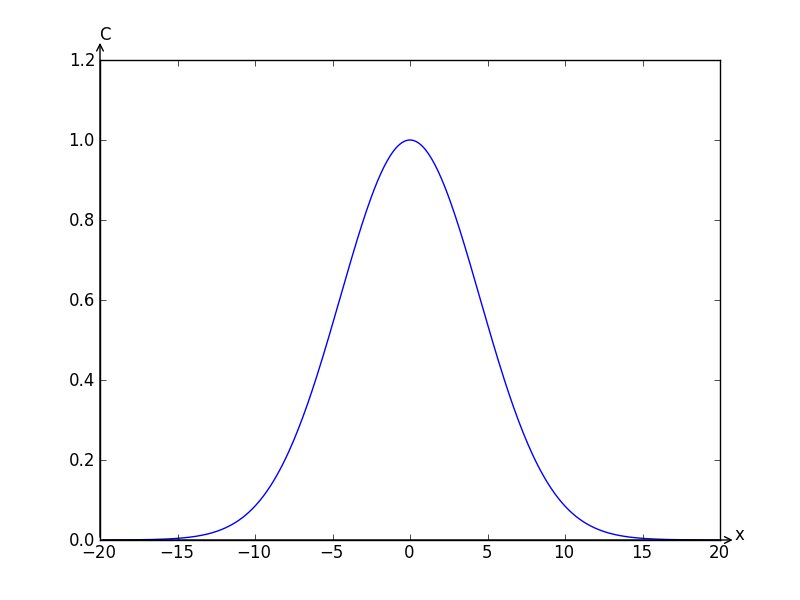
\includegraphics[width=0.5\linewidth]{img/twoCylinders.png}
		\caption{Зависимость коэффициента передачи двух одинаковых волноводов с радиусом моды 4~мкм}
\end{figure}
\begin{figure}[h!]
		\includegraphics[width=0.5\linewidth]{img/twoCylinders2.png}
		\caption{Зависимость коэффициента передачи двух волноводов с радиусами моды 4~мкм и 7~мкм}
\end{figure}

\newpage
\section{Интерактивная модель}

Кроме статических графиков, была построена модель, позволяющая быстро и просто находить вид выходного распределения.

Слева показывается расчитанное распределение поля в выодном волноводе. В правой части схематично показывается перекрытие полей мод. Ниже показаны числовые значения рассчитываемых параметров. Кликами по распределению поля можно изменять вид перекрытия и изображение будет перестраиваться, показывая новое распределение. Эту модель удобно использовать для моделирования экспериментов, задавая значения и сразу же получая результат.

\begin{figure}[h!]
	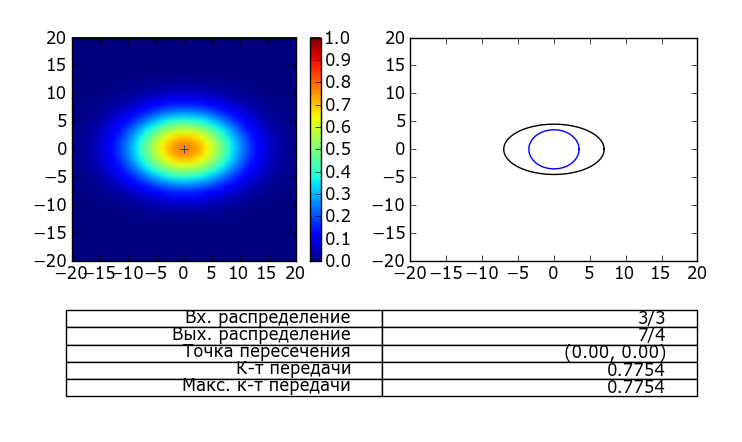
\includegraphics[width=\linewidth]{img/heatmap.png}
	\caption{Общий вид программы}
\end{figure}